\documentclass{article}%
\usepackage[T1]{fontenc}%
\usepackage[utf8]{inputenc}%
\usepackage{lmodern}%
\usepackage{textcomp}%
\usepackage{lastpage}%
\usepackage{authblk}%
\usepackage{graphicx}%
%
\title{Involvement of Nrf2{-}Mediated Upregulation of Heme Oxygenase{-}1 in Mollugin{-}Induced Growth Inhibition and Apoptosis in Human Oral Cancer Cells}%
\author{Curtis Gilbert}%
\affil{School of Dentistry, Chung Shan Medical University, Taichung 40201, Taiwan}%
\date{01{-}01{-}2006}%
%
\begin{document}%
\normalsize%
\maketitle%
\section{Abstract}%
\label{sec:Abstract}%
As is obvious, liver cells start producing enzymes when a liver is compromised. For some diseases and cancers, if liver cells dont start making enzymes, they eventually start to get sick.\newline%
This condition is called interferon{-}a2b{-}induced apoptosis, or IAP. When this cell is damaged, it becomes myocardial enucleation (MEE). When the enzyme keeps up, it sends electrical impulses to the liver that trigger apoptosis. This goes on for long periods without impacting the cells ability to produce the enzyme. These neurons are also triggered by increased inflammation of the liver.\newline%
Hematic enucleation reduces the toxin, which produces other drugs, called fibrotic proteins, that halt the apoptosis process in a cellular level. This ultimately results in fewer genetic glitches in some cases.\newline%
Interferon{-}a2b{-}induced apoptosis has been known for some time, but we did not even know it would be the underlying cause of these results, says an author of a study published in the journal Hepatology.\newline%
The following detailed information about this study can be found in the preprint page of the article.

%
\subsection{Image Analysis}%
\label{subsec:ImageAnalysis}%


\begin{figure}[h!]%
\centering%
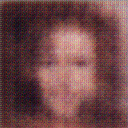
\includegraphics[width=150px]{500_fake_images/samples_5_43.png}%
\caption{A Man Is Taking A Picture Of Himself In A Mirror}%
\end{figure}

%
\end{document}